% !TeX spellcheck = en_US
\documentclass[aspectratio=1610]{beamer}
\usetheme{Madrid}
\setbeamercovered{transparent}
\setbeamertemplate{navigation symbols}{}
\setbeamertemplate{itemize items}[circle]
\setbeamertemplate{enumerate items}[default]

\makeatletter
\define@key{beamerframe}{wide}[10pt]{%
	\def\beamer@cramped{\itemsep #1\topsep0.5pt\relax}}
\makeatother


\usepackage[english]{babel}
\usepackage[utf8]{inputenc}
\usepackage[T1]{fontenc}
\usepackage{array}

\title[Fall - Lecture 1] % (optional, use only with long paper titles)
{Intermediate Macroeconomics: Lecture  1 (Ch.1)}
\subtitle{ECON 311 -- Intermediate Macroeconomics}

\author{Muhebullah Karimzada}
\institute{School of Economics \\\ University of Northern British Columbia}
\date{Fall 2026}


% ---------- UNBC COLORS ----------
\usepackage{xcolor}
\definecolor{UNBCGreen}{RGB}{0,102,51}
\definecolor{UNBCDark}{RGB}{0,74,37}
\definecolor{UNBCGold}{RGB}{189,155,96}
\definecolor{SoftCream}{RGB}{249,247,242}
\definecolor{SoftGray}{RGB}{244,246,248}
\definecolor{AccentBlue}{RGB}{41,98,255}
\definecolor{AccentOrange}{RGB}{230,126,34}
\definecolor{AccentTeal}{RGB}{0,150,136}
\definecolor{AccentRed}{RGB}{192,57,43}
\setbeamercolor{normal text}{fg=black,bg=white}
\setbeamercolor{structure}{fg=UNBCDark}
\setbeamercolor{title}{fg=white,bg=UNBCDark}
\setbeamercolor{subtitle}{fg=UNBCGold}
\setbeamercolor{frametitle}{fg=white,bg=UNBCDark}
\setbeamercolor{block title}{fg=white,bg=UNBCDark}
\setbeamercolor{block body}{fg=black,bg=SoftGray}
\setbeamercolor{block title alerted}{fg=white,bg=AccentRed}
\setbeamercolor{block body alerted}{fg=black,bg=SoftGray}
\setbeamercolor{item}{fg=UNBCDark}
\setbeamercolor{section in toc}{fg=UNBCDark}
\setbeamercolor{alerted text}{fg=AccentRed}
\setbeamercolor{author in head/foot}{fg=white,bg=UNBCDark}
\setbeamercolor{date in head/foot}{fg=white,bg=UNBCDark}
% ---------- UNBC BRANDING ----------
\usepackage{graphicx}
\usepackage{lmodern}
\usepackage{tcolorbox}
\usepackage{tikz}
\usetikzlibrary{positioning,calc}
\setbeamertemplate{headline}{}
\setbeamertemplate{footline}{%
  \leavevmode%
  \hbox{%
  \begin{beamercolorbox}[wd=.78\paperwidth,ht=2.8ex,dp=1.2ex,leftskip=1em]{author in head/foot}%
  \color{white}\textbf{ECON 311} \hspace{0.5em} \textcolor{UNBCGold}{|} \hspace{0.5em} Intermediate Macroeconomics%
  \end{beamercolorbox}%
  \begin{beamercolorbox}[wd=.22\paperwidth,ht=2.8ex,dp=1.2ex,rightskip=1em plus1fil]{date in head/foot}%
  \color{white}\insertframenumber/\inserttotalframenumber%
  \end{beamercolorbox}}%
}

\newtcolorbox{mybox}[2][]{
  colback=#2!8,
  colframe=#2,
  boxrule=0.8pt,
  arc=2mm,
  left=2mm,right=2mm,top=1.5mm,bottom=1.5mm,
  #1
}

\newcommand{\topbanner}[1]{%
\begin{tikzpicture}[remember picture,overlay]
\fill[UNBCGold] ([yshift=-0.65cm]current page.north west) rectangle ([yshift=-0.48cm]current page.north east);
\node[anchor=north west,font=\small\bfseries,text=UNBCDark] at ([xshift=0.35cm,yshift=-0.78cm]current page.north west) {#1};
\end{tikzpicture}%
}
\begin{document}

\begin{frame}[plain]
  \titlepage
\end{frame}





\begin{frame}[wide]{Textbook}
	\begin{itemize}
		\item We are going to follow the textbook for the majority of the course
		\item Textbook: \textit{Macroeconomics, by Charles I. Jones, 5th edition}
	\end{itemize}
	\begin{figure}
		\centering
		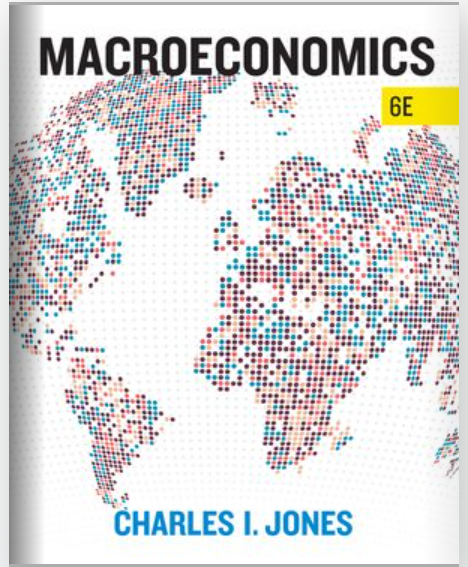
\includegraphics[width=0.3\linewidth]{Figures/textbook}
	\end{figure}
\end{frame}
\begin{frame}[wide]{What are You Going to Learn (ch. 1)}
	\begin{itemize}
		\item What are the important macroeconomics questions to be considered	
		\item The three-part structure of the course/textbook:
		\begin{itemize}
			\item The long run
			\item The short run
			\item Issues for the future
		\end{itemize}
		\item Foundations of macroeconomic models and modeling
	\end{itemize}
\end{frame}

\begin{frame}[wide]{Important Macroeconomic Questions to Consider}
	Long-run questions:
	\begin{itemize}
		\item Why is today’s average North American
		\begin{itemize}
			\item more than 10 times richer than 100 years ago?
			\item 50 times richer than the average Ethiopian?
		\end{itemize}
		\item What could be the cause of high income inequality across the world and even within a single country?
		%		\begin{itemize}
			%			\item Is it equitable that such a small percentage of people control such a large percent of the world’s wealth?
			%		\end{itemize}
		\item Why has the unemployment rate in Europe been almost twice as high as it has been in the United States?
	\end{itemize}
\end{frame}

\begin{frame}[wide]{Important Macroeconomic Questions to Consider}
	Short-run questions:
	\begin{itemize}
		\item Do we understand and know the causes of the global financial crisis in 2007-2008
		\begin{itemize}
			\item Was it greedy banks lending money, irresponsible homeowners living beyond their means, or government institutions such as Freddie Mac and Fannie Mae? 
		\end{itemize} 
		\item What are the causes of the recent rise in prices?
		\item How did the 2008 Affordable Care Act impact the price of healthcare, economic growth, and government expenditures?
	\end{itemize}
\end{frame}

\begin{frame}[wide]{GDP Per Capita Across Regions }
	\begin{itemize}
		\item GDP Per Capita  represents the average income per individual in a country
		\item GDP per Capita is much higher in developed countries (Western Europe and Western Offshoots - North America \& Australia \& New Zealand) compared to the rest
		\item Asia, Eastern Europe and Middle East experience an uptick in recent years
	\end{itemize}
	\begin{figure}
		\centering
		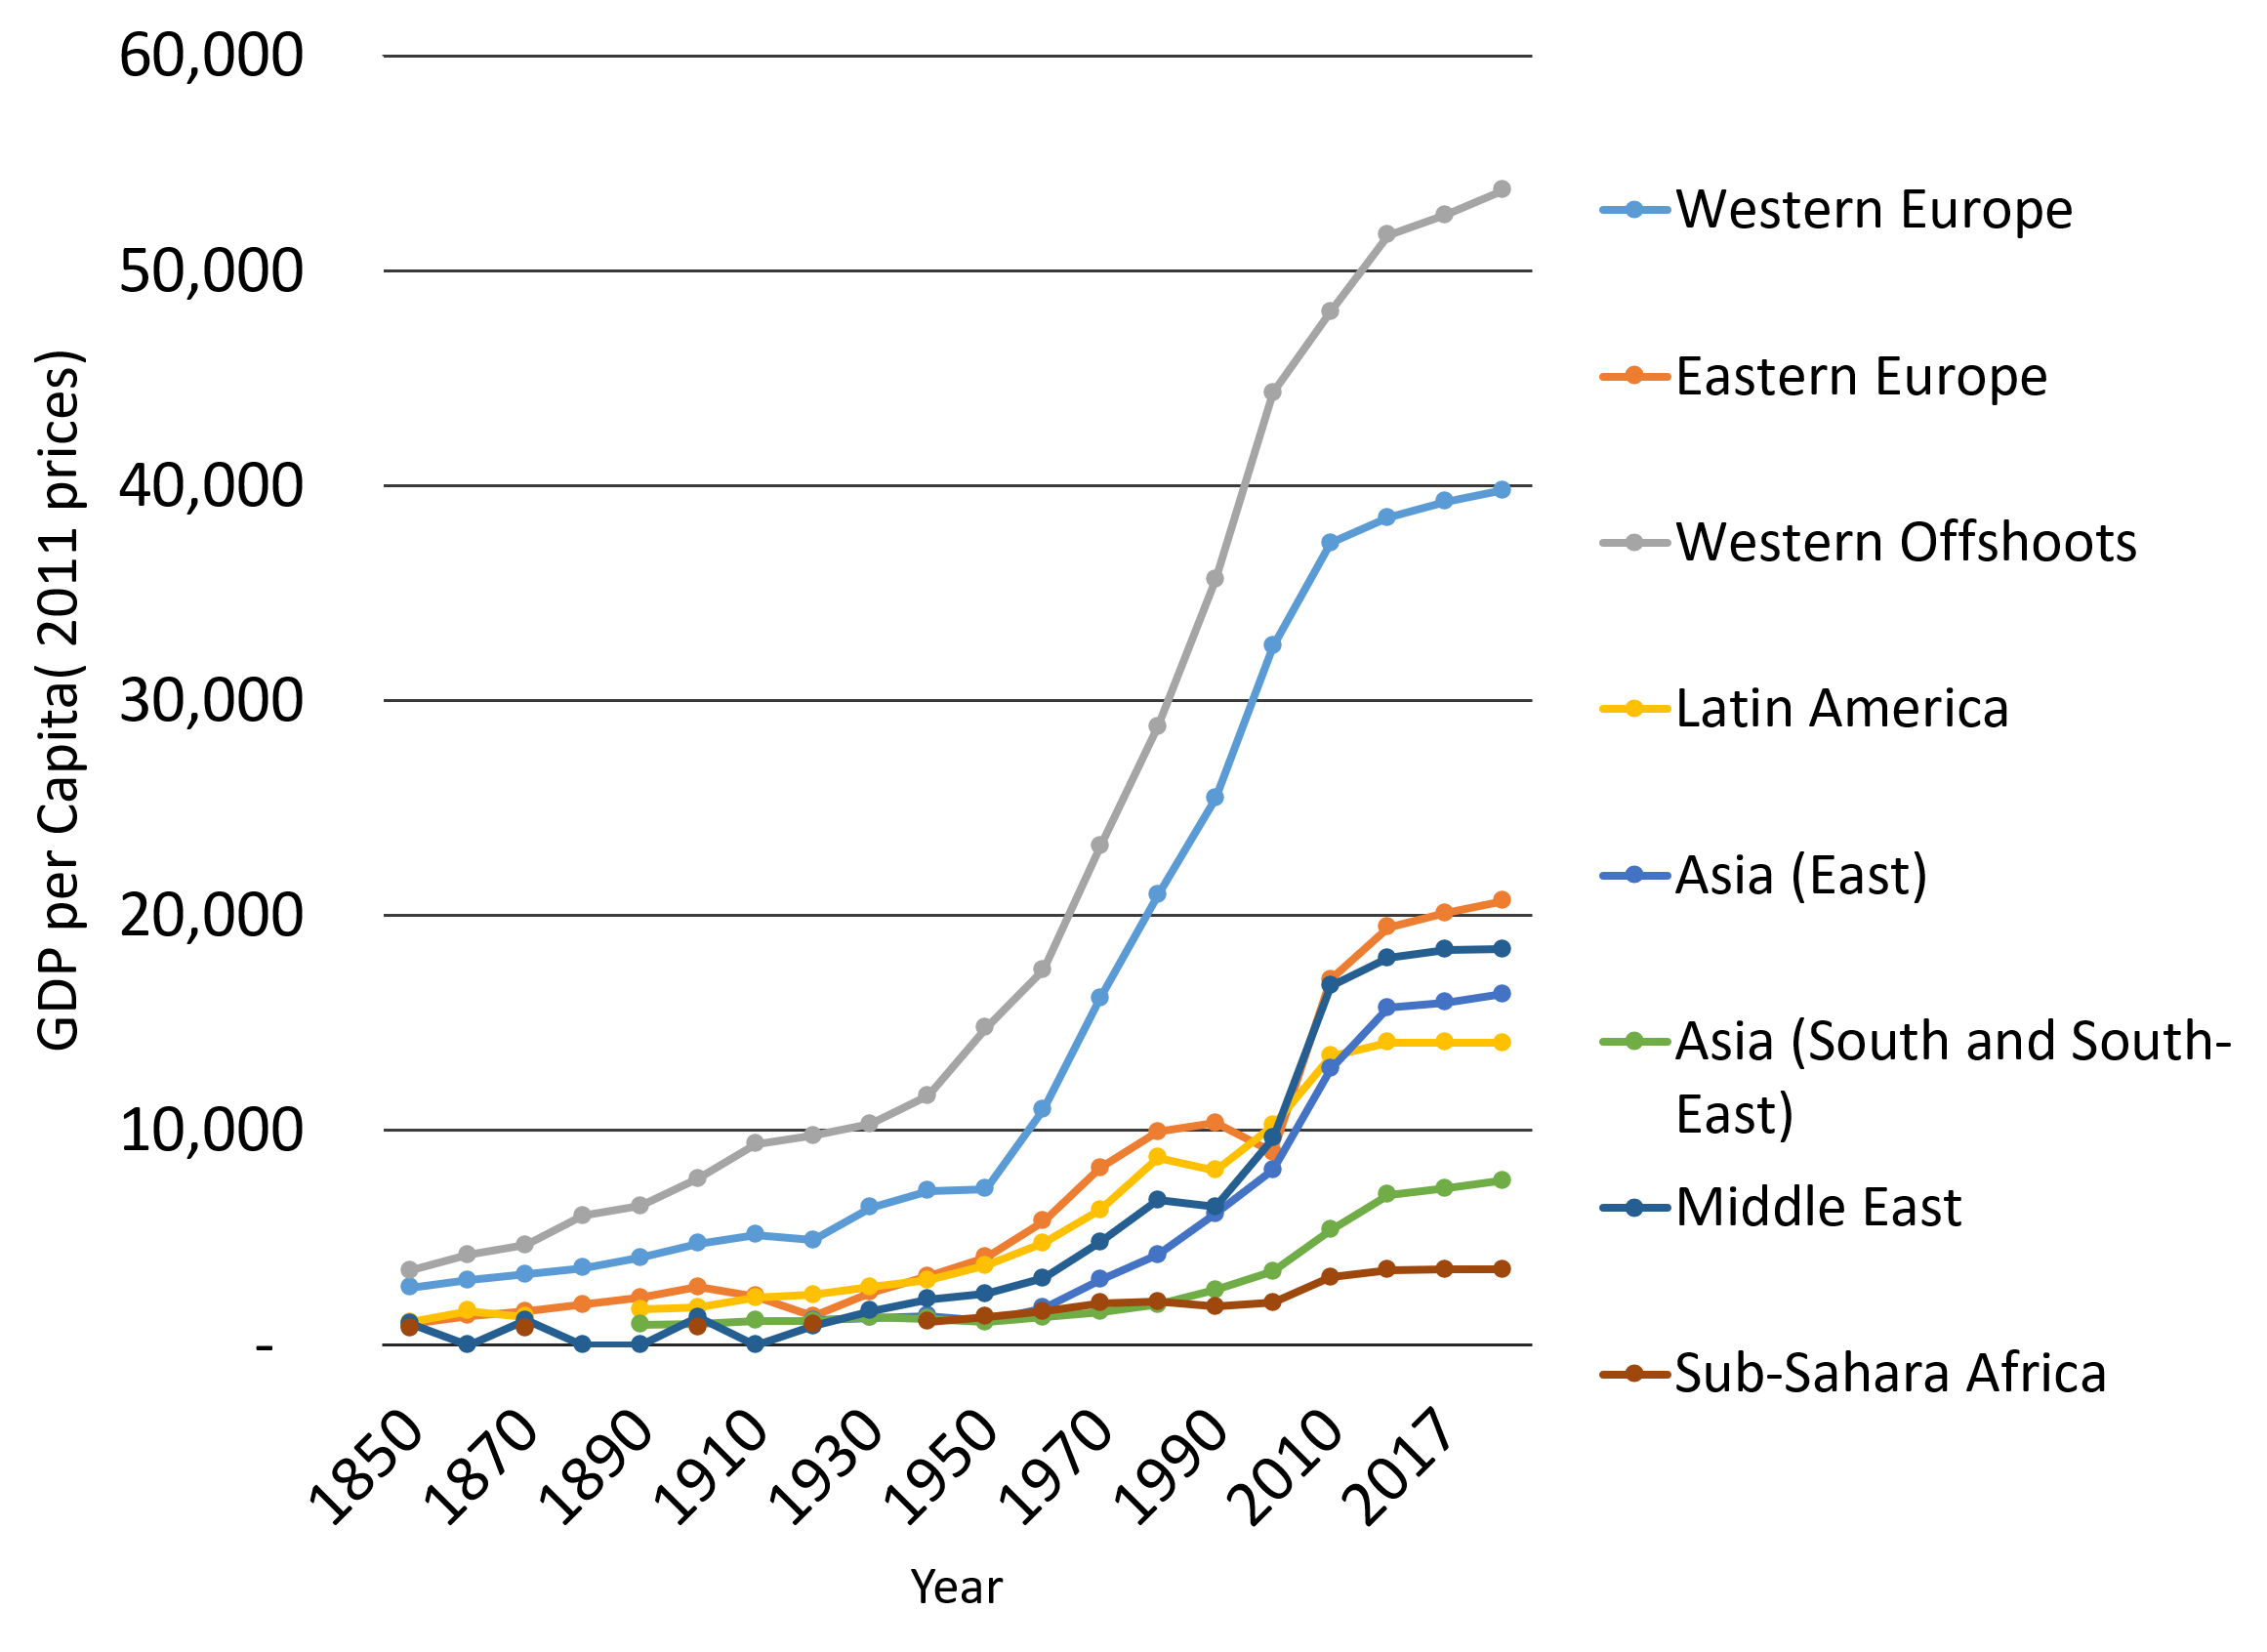
\includegraphics[width=0.55\linewidth]{Figures/econ_growth}
	\end{figure}
	
\end{frame}

\begin{frame}[wide]{The Long Run}
	\begin{itemize}
		\item Income per person in the United States:
		\begin{itemize}
			\item \$2,800 in 1870
			\item \$44,000 in 2008
			\item \$76,000 in 2025
		\end{itemize}
		\item As seen earlier, many countries have not experienced similar increases in living standards
		\item The analysis of economic growth helps explain the long run
	\end{itemize}
\end{frame}

\begin{frame}[wide]{Per Capita GDP in the United States, 1870–2015}
	\begin{itemize}
		\item Overall growth is upward
		\item Short-run fluctuations can cause peaks and troughs
		\item It encourages us to ask, Will there ever be a long-run peak? Can we grow forever? What does the future hold?
	\end{itemize}
	\begin{figure}
		\centering
		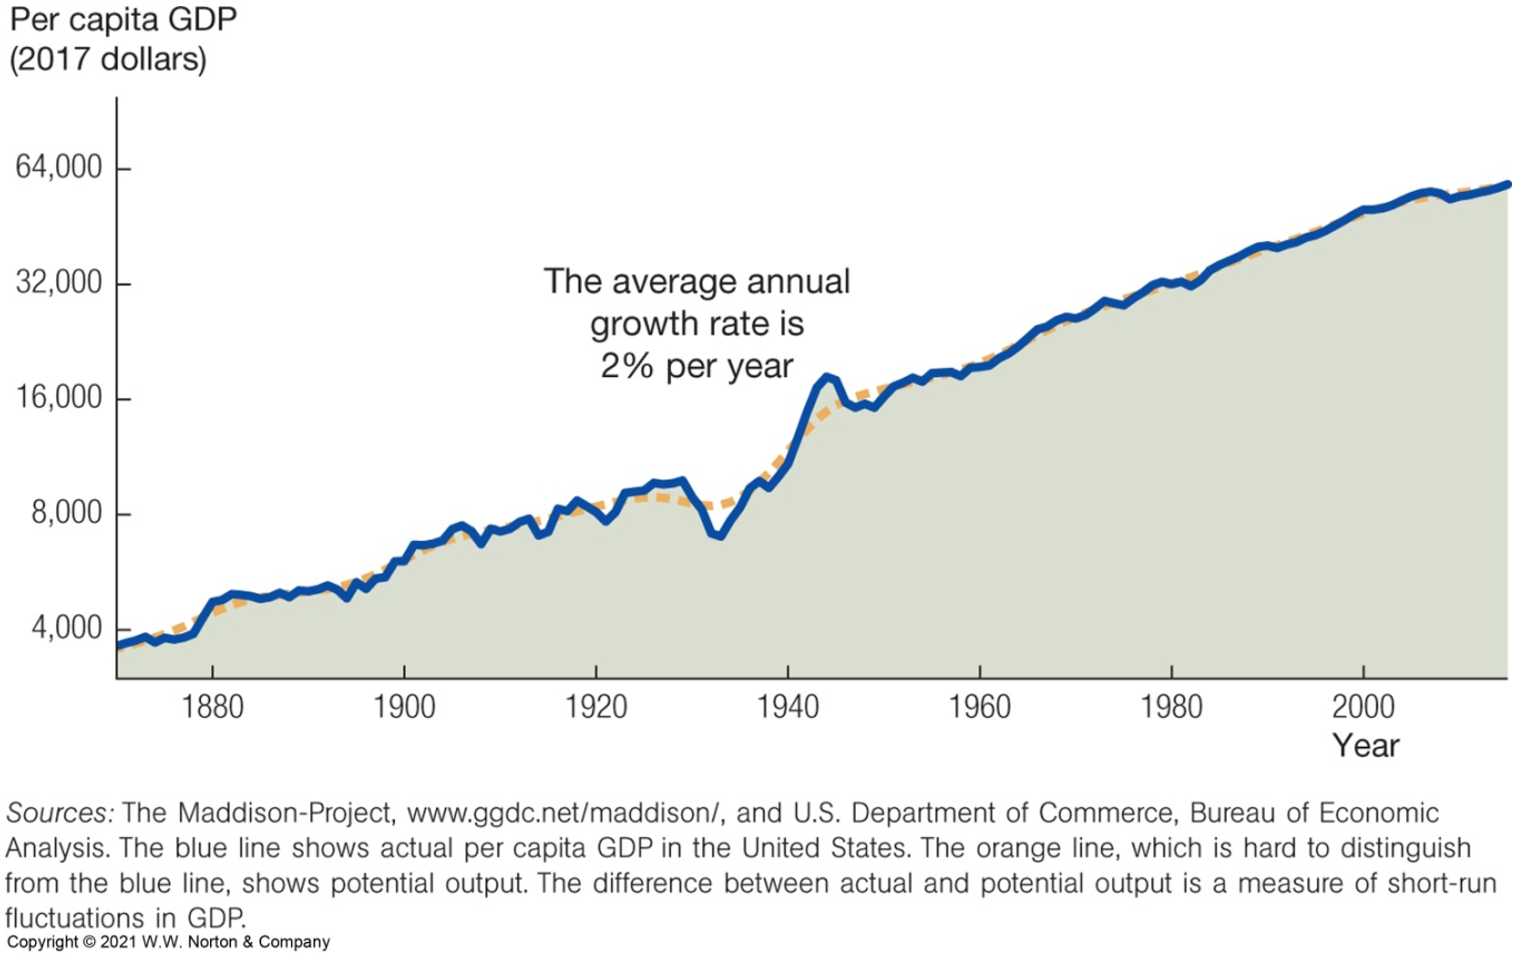
\includegraphics[width=0.55\linewidth]{Figures/per_capita_GDP_US_1870-2015}
	\end{figure}
	
\end{frame}

%\begin{frame}[wide]{Economic Growth}
%	\begin{itemize}
	%		\item Economists develop mathematical models to study these phenomena
	%		\begin{itemize}
		%			\item For example, why do some countries grow faster than others?
		%		 	\item To answer this question, we will use the Solow growth model and a model of endogenous growth
		%		 	\item We are going explore these in the first half of the course
		%		\end{itemize}
	%		
	%	\end{itemize}
%\end{frame}

\begin{frame}[wide]{The Short Run}
	\begin{itemize}
		\item Potential output $(Y_p)$: Measure of how per capita GDP would evolve with completely flexible prices and fully employed resources
		\item Short-run fluctuations are often defined as deviations of actual output (Y) from its potential level
		\begin{itemize}
			\item When $Y > Y_p$, this is an expansion
			\item When $Y < Y_p$, this is a recession
		\end{itemize}
		\item In 1982, actual output was 5 percent less than potential output, which is economically important 
		\begin{itemize}
			\item In today’s prices, the gap was roughly \$1,500 per person (\$6,000 for a typical family of 4)
			\item This recession represented a large cost in terms of lost income
		\end{itemize}
		\item Recessions are costly and cause devastation in the short run but are overcome by long-run trends
	\end{itemize}
\end{frame}

\begin{frame}[wide]{Inflation Rate in Certain Developed Countries}
	\begin{itemize}
		\item The inflation rate is the percentage change in the price level -- often measured using CPI
	\end{itemize}
	\begin{figure}
		\centering
		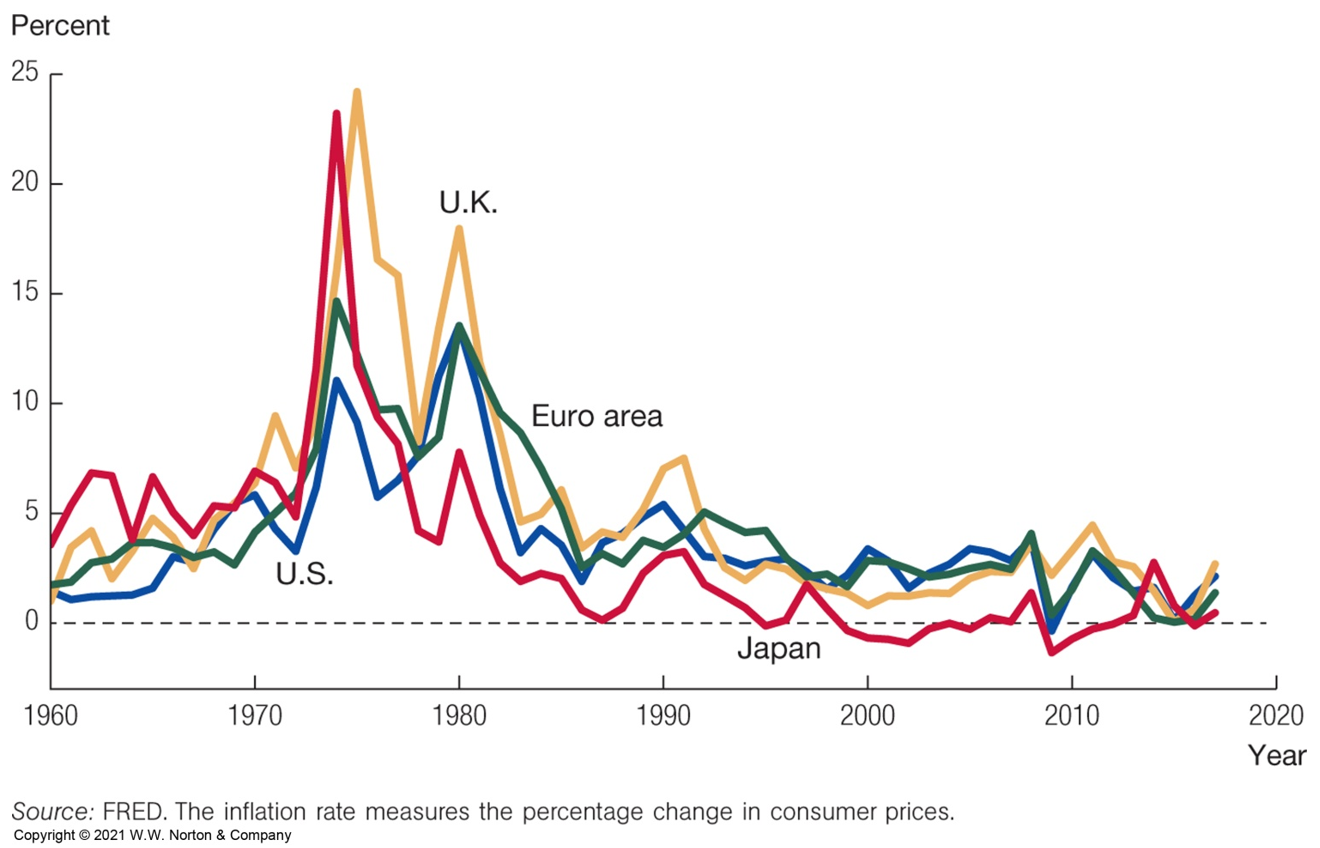
\includegraphics[width=0.65\linewidth]{Figures/inflation_across_countries}
	\end{figure}
	
\end{frame}


\begin{frame}[wide]{The Unemployment Rate in the United States, Europe, and Japan}
	\begin{itemize}
		\item Unemployment rate are highly correlated with the business cycle
		\item Before 1980, unemployment rates in Europe were actually lower than in the United States, while Japan has remained low over this time frame
	\end{itemize}
	\begin{figure}
		\centering
		\includegraphics[width=0.5\linewidth]{"Figures/Unemployment Rate"}
	\end{figure}
\end{frame}

%\begin{frame}[wide]{News on Inflation}
%	\begin{itemize}
	%		\item News on Inflation appear almost every weeks
	%	\end{itemize}
%	\begin{figure}
	%		\centering
	%		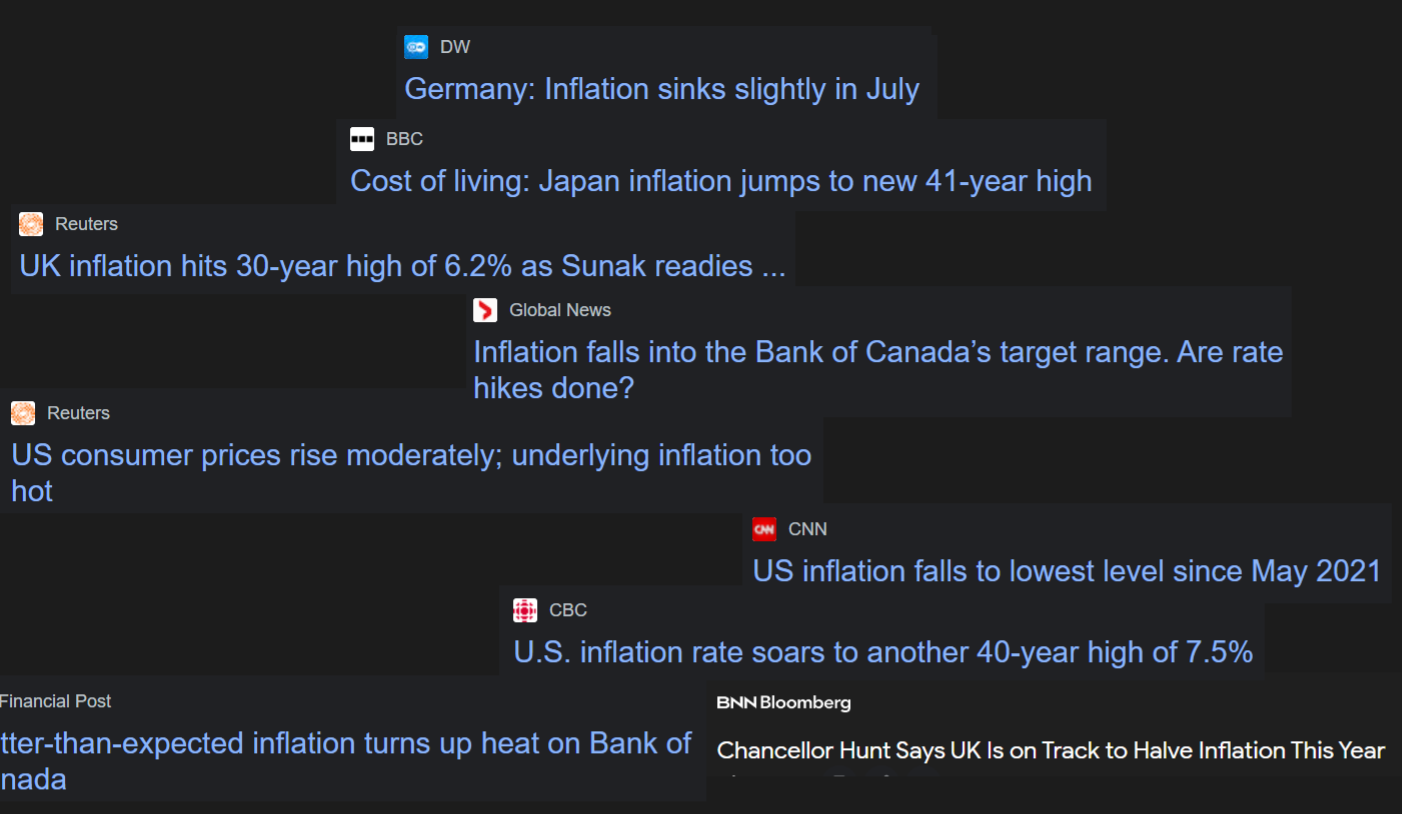
\includegraphics[width=0.7\linewidth]{Figures/inflation_news}
	%	\end{figure}
%
%\end{frame}
%
%\begin{frame}[wide]{What are the costs of inflation to society?}
%	\begin{itemize}
	%		\item Unexpected and symmetric inflation
	%		\begin{itemize}
		%			\item Wages are simply the price of labor
		%			\item Therefore, purchasing power of workers is unaffected,	in this case, no one is worse off
		%			
		%		\end{itemize}
	%		\item Unexpected and asymmetric inflation
	%		\begin{itemize}
		%			\item Suppose wages increase less than the prices for goods and services
		%			\item In this case, workers are worse off and relative price distortions emerge
		%			\item Unexpected and uneven inflation is generally costly to society
		%		\end{itemize}
	%	\end{itemize}
%\end{frame}
%
%\begin{frame}[wide]{What are the costs of inflation to society?}
%	\begin{itemize}
	%		\item  Deflation
	%		\begin{itemize}
		%			\item Deflation increases the real value of outstanding debt, this is harmful to borrowers and restricts access to credit
		%			\begin{itemize}
			%				\item Firm also earn less in dollar term but might hold same amount of debt
			%			\end{itemize}
		%			\item Consumer form an expectation that the price would keep falling
		%		\end{itemize}
	%		\item Sticky prices
	%		\begin{itemize}
		%			\item Sticky prices are related to the asymmetric (uneven) inflation
		%			\item If some prices do not adjust as quickly as others, there are resulting distortions and inefficiencies
		%			\item Distortions are bad—see end of the lecture—Pareto efficiency and free markets
		%			\item Sticky prices cause inflation to be costly
		%		\end{itemize}
	%	\end{itemize}
%\end{frame}


\begin{frame}[wide]{An Overview of the Course }
	\begin{itemize}
		\item Microeconomics also has many subfields and a lot of them are overlapped with macroeconomics
	\end{itemize}
	\begin{figure}
		\centering
		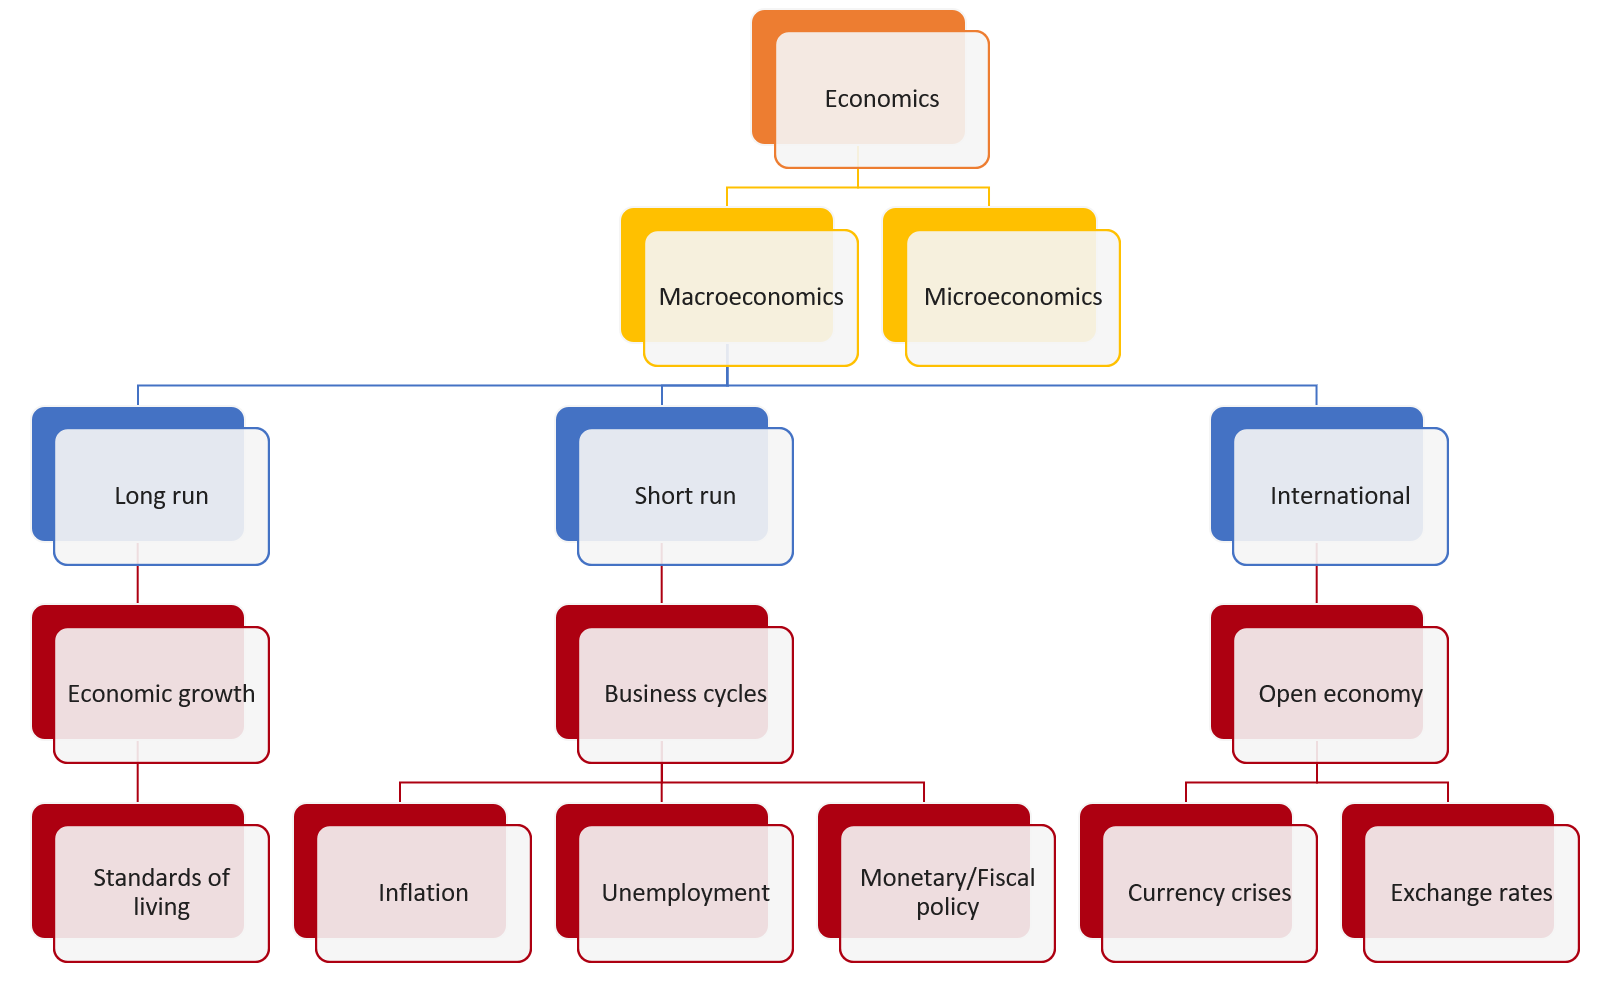
\includegraphics[width=0.7\linewidth]{Figures/overview}
	\end{figure}
	
\end{frame}







\begin{frame}[wide]{How Macroeconomics Studies Key Questions}
	Macroeconomists have a general approach to study questions of interest:
	\begin{itemize}
		\item Document the facts
		\begin{itemize}
			\item In recent years, more macroeconomists rely more and more on micro-data
		\end{itemize}
		\item Develop a model
		\begin{itemize}
			\item Models simplify the complicated real world into its most relevant elements
			\begin{itemize}
				\item The goal of a model is not to perfectly replicate every single detail/feature of markets or behavior
			\end{itemize}
			\item A model is useful if it has good predictive power
			\item Economic models often involve systems of multiple equations
		\end{itemize}
		\item Compare predictions of the model with original facts
		\item Use the model to make other predictions that will eventually be tested
	\end{itemize}
\end{frame}

\begin{frame}[wide]{Parts of an Economic Model}
	\begin{itemize}
		\item Parameter: An input that is fixed over time, except when the model builder changes it for an experiment
		\begin{itemize}
			\item Minimum we assume not to change; can be changed by the model builder as an experiment			
		\end{itemize}
		\item Exogenous variable: An input that can change over time, but determined ahead of time by the model builder
		\begin{itemize}
			\item Exogenous = “outside of the model”
			\item Can change over time but determined outside of the model.
			
		\end{itemize}
		\item Endogenous variable: An outcome of the model—something that is explained by the model
		\begin{itemize}
			\item Endogenous = “within the model”
			\item Determined by factors plugged into our model.
		\end{itemize}
		
	\end{itemize}
\end{frame}

\begin{frame}[wide]{Parts of an Economic Model}
	
	\begin{figure}
		\centering
		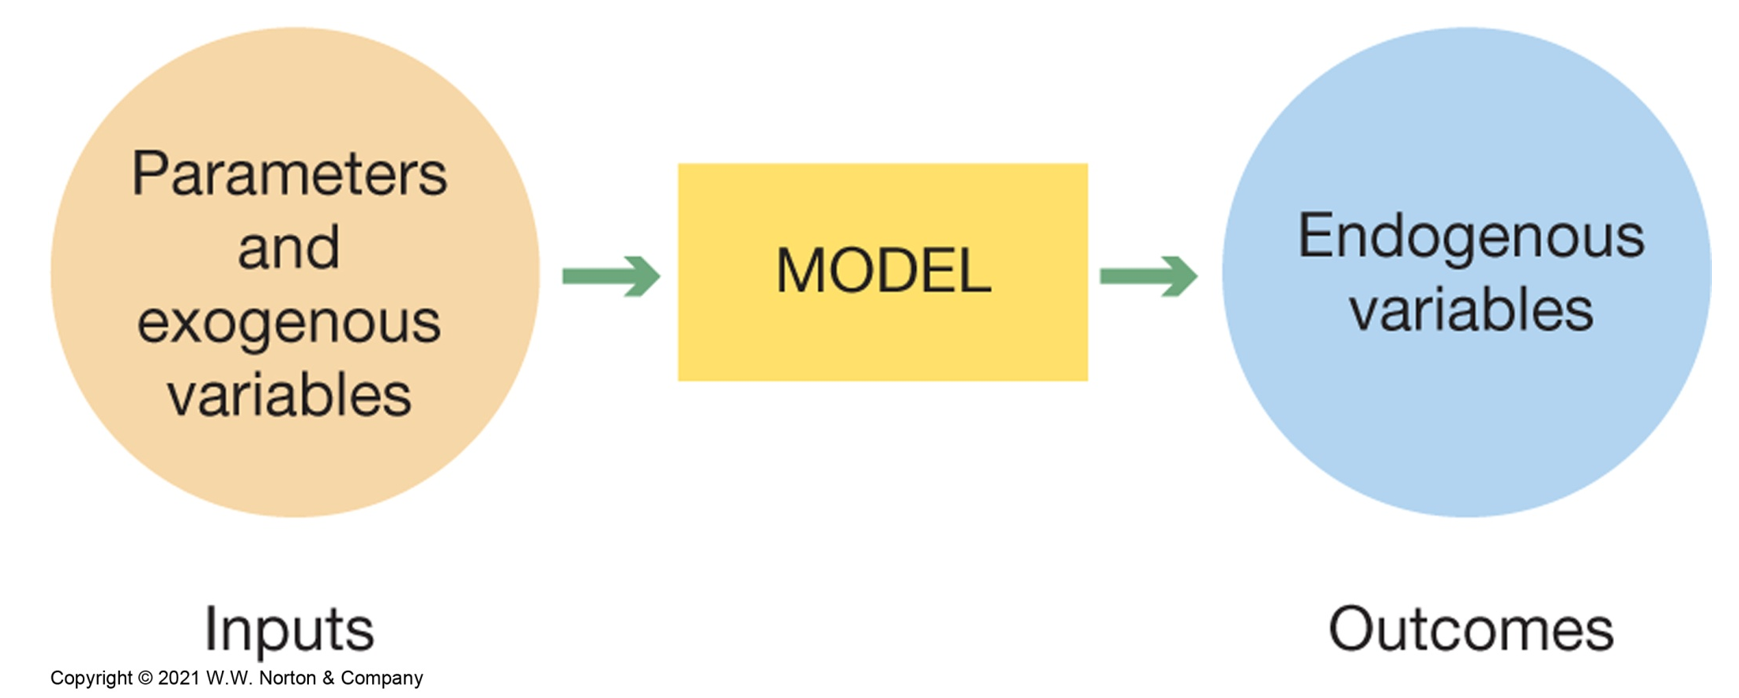
\includegraphics[width=0.6\linewidth]{Figures/model_part}
	\end{figure}
	\begin{itemize}
		\item For example, a linear model
		\[Y = \beta_0 + \beta_1 X_1 + \beta_2 X_2 \]
	\end{itemize}
\end{frame}

\begin{frame}[wide]{Suppose We Have a Working Model…}
	\begin{itemize}
		\item How can we use it?
		\begin{itemize}
			\item Models are built using existing data, but can be used to predict events and outcomes for which we do not have data yet -- set up a counterfactual “what if” situation
			\item Change parameters and exogenous variables to see how they affect endogenous variables
			\item Predict costs and benefits of new government policies -- a change in parameter that mimic the policy
			\item All models can make inaccurate predictions, so we should always interpret the results with caution			
		\end{itemize}
	\end{itemize}
\end{frame}

\begin{frame}[wide]{Model Example: Labor supply and demand}
	\begin{itemize}
		\item Variables:
		\begin{itemize}[]
			\item $L_s = $ number of hours laborers want to work
			\item $L_D = $ number of labor hours firms want to hire
			\item $w = $ wage
		\end{itemize} 		
		\item no exogenous variables
		\item Parameter: $\bar{f}$, $\bar{l}$, $\bar{a}$
	\end{itemize}
\end{frame}

\begin{frame}[wide]{Model Example: Labor supply and demand}
	\begin{columns} 
		% Column 1
		\begin{column}{.5\textwidth}
			\begin{itemize}
				\item Supply Function: 
				\[L_s = f(w) = \bar{a}w + \bar{l} = 2w+30\]
				\item Demand Function:
				\[L_d = g(w) = \bar{f} - w = 60-w\]
				\item Equilibrium:
				\[L_d = L_s\]
			\end{itemize}	
		\end{column}
		% Column 2    
		\begin{column}{.5\textwidth}
			\begin{figure}
				\centering
				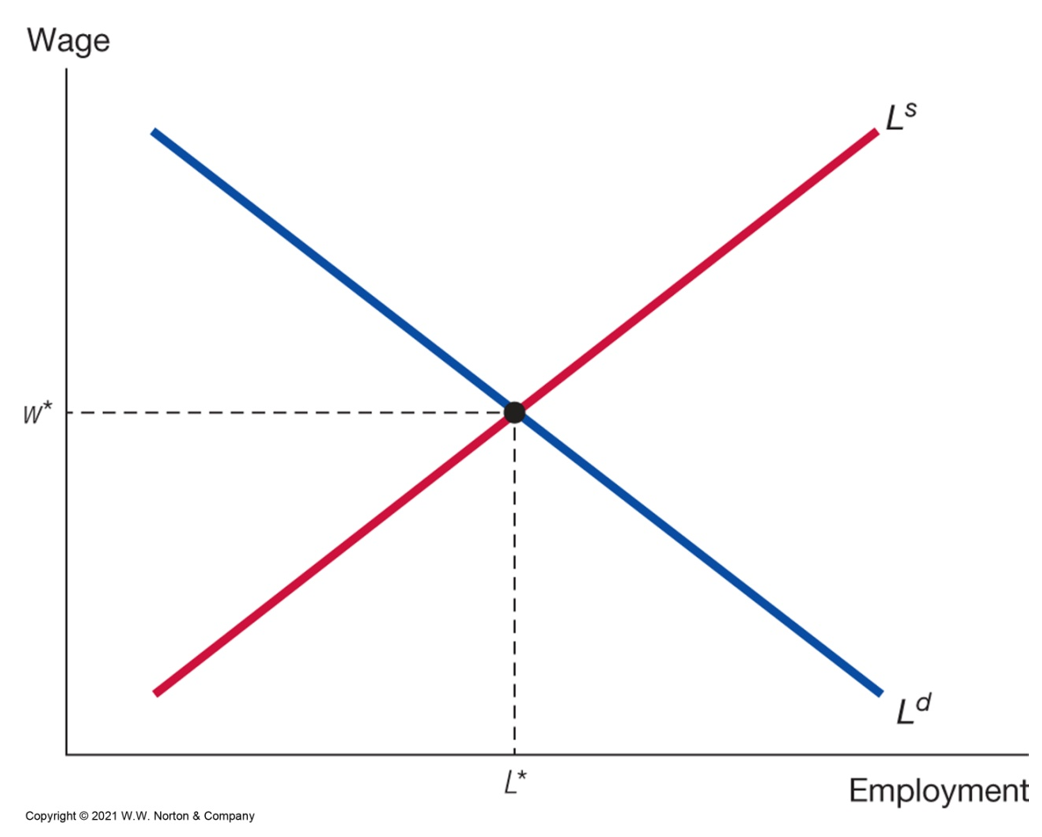
\includegraphics[width=0.7\linewidth]{Figures/labor_mkt_eqm}
			\end{figure}
			
		\end{column}%
	\end{columns}
\end{frame}


\begin{frame}[wide]{Model Example: Labor supply and demand}
	\begin{itemize}
		\item Consider a case of an increase in income taxes
		\item Firm would still pays a wage of $w$, but worker receives only a wage of $(1 - t)w$
		\item For any given wage, the worker gets to keep less of his wage so he supplies less labor. In equilibrium, we move from $(w^*,L^*)$ to $(w^{*'},L^{*'})$
	\end{itemize}
	\begin{figure}
		\centering
		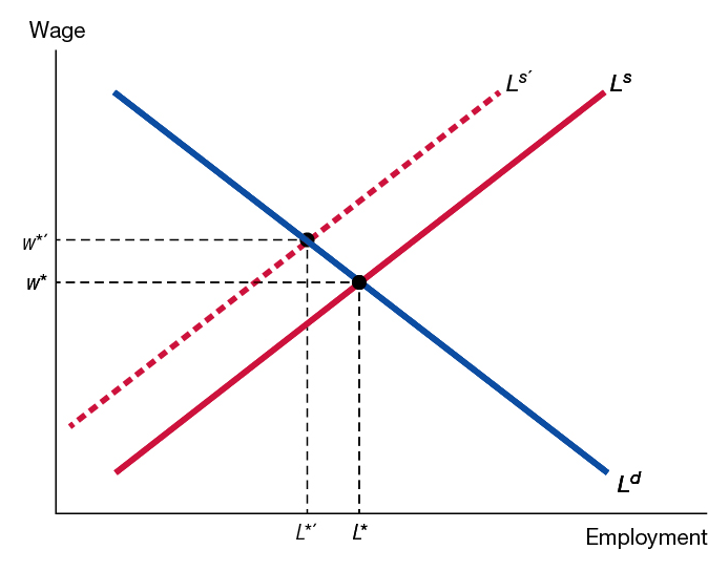
\includegraphics[width=0.45\linewidth]{Figures/labor_mkt_eqm2}
	\end{figure}
	
\end{frame}

\begin{frame}[wide]{Model Example: Labor supply and demand}
	\begin{itemize}
		\item Consider a case of an increase in an input price
		\item As production costs increase for firms, their demand for labor decreases. It lead to a leftward shift in $L_d$
		\item The equilibrium move from  $(w^*,L^*)$ to $(w^{*'},L^{*'})$
	\end{itemize}
	\begin{figure}
		\centering
		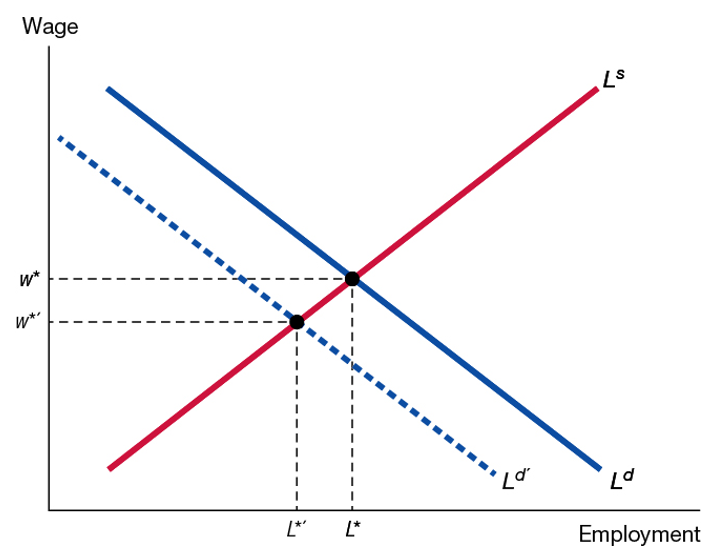
\includegraphics[width=0.45\linewidth]{Figures/labor_mkt_eqm3}
	\end{figure}
	
\end{frame}

%\begin{frame}[wide]{Theoretical and Empirical Approach}
%	\begin{itemize}
	%		\item They rely on each other to solidify the validity of analyses
	%		\item Most mainstream theoretical methods are motivated by empirical work, theoretical models typically try to explain some important feature of the data
	%		\item Empirical macroeconomics needs theoretical macroeconomics to establish causation
	%		\begin{itemize}
		%			\item Suppose the data show that when interest rates decrease, taxes usually go down
		%			\item It might be tempting to conclude that reduced interest rates lead to decreased taxes. However, this can go the other way around
		%			\item Or,  there is likely omitted variable bias here, which implies that a third variable is causing the changes in both interest rates and taxes
		%			\item For instance, poor macroeconomic conditions probably result in the central bank decreasing interest rates and the government cutting taxes
		%		\end{itemize}
	%		\item Empirical work can never establish causality with 100 percent probability. But, when it is supported by theory, a causal relationship is more convincing
	%	\end{itemize}
%\end{frame}


%\begin{frame}[wide]{Welfare}
%	\begin{itemize}
	%		\item Welfare: Variable used to determine preferable policies and rank outcomes
	%		\item Measuring welfare is highly subjective
	%		\begin{itemize}
		%			\item More GDP (consumption) increases welfare
		%		\end{itemize}
	%		\item Are there variables other than GDP that we should consider?
	%		\begin{itemize}
		%			\item Leisure
		%			\item Equality
		%			\item Life expectancy
		%			\item Environmental quality
		%			\item Individual freedom
		%		\end{itemize}
	%		\item Often, policymakers use increasing GDP as a benchmark for standards of living and welfare
	%	\end{itemize}
%\end{frame}
%
%\begin{frame}[wide]{Pareto Efficiency and Free Markets}
%	\begin{itemize}
	%		\item How do efficiency can be measure in term of welfare?
	%		\item Pareto efficiency is reached when you cannot make someone else better off without making another worse off
	%		\item The fundamental theorem of welfare economics (a version of Adam Smith’s invisible hand) states if there is a competitive market for everything, then equilibrium will be Pareto efficient
	%		\item However, if complete and competitive markets do not exist there is no reason to believe that equilibrium will be Pareto efficient
	%		\item Deviations:
	%		\begin{itemize}
		%			\item Market power
		%			\item Externalities
		%			\item Public goods
		%			\item Asymmetric (imperfect) information
		%		\end{itemize}
	%		
	%	\end{itemize}
%\end{frame}

%\begin{frame}[wide]{Why do economists disagree?}
%	\begin{itemize}
	%		\item Nature of market failures (magnitude)
	%		\item Theory of complete and competitive markets breaks down
	%		\item Which Pareto efficient outcome is best?
	%		
	%	\end{itemize}
%\end{frame}


\begin{frame}[wide]{Next Lecture}
	\begin{itemize}
		\item Next lecture will cover Ch.2
	\end{itemize}
\end{frame}

\end{document}